In order to test the grid point and connectivity algorithms, 
we use this simple $4\times 3$ element mesh:

\begin{verbatim}

      Q_2 X Q1 (serendipity)                    Q_2 X Q_1 (regular)

15--47--16--48--17--49--18--50--19      54--55--56--57--58--59--60--61--62
 |       |       |       |       |       |   :   |   :   |   :   |   :   |
42      43      44      45      46      45..46..47..48..49..50..51..52..53
 |       |       |       |       |       |   :   |   :   |   :   |   :   |
10--38--11--39--12--40--13--41--14      36--37--38--39--40--41--42--43--44
 |       |       |       |       |       |   :   |   :   |   :   |   :   |
33      34      35      36      37      27..28..29..30..31..32..33..34..35
 |       |       |       |       |       |   :   |   :   |   :   |   :   |
05--29--06--30--07--31--08--32--09      18--19--20--21--22--23--24--25--26
 |       |       |       |       |       |   :   |   :   |   :   |   :   |
24      25      26      27      28      09..10..11..12..13..14..15..16..17
 |       |       |       |       |       |   :   |   :   |   :   |   :   |
00--20--01--21--02--22--03--23--04      00--01--02--03--04--05--06--07--08
\end{verbatim}

We see that the serendipity element-based mesh counts only 51 nodes, as
opposed to 63 for its counterpart.

Setting $nelx=nely$, we can look at the number of velocity nodes for each 
as a function of $nelx$, as shown hereunder:

\begin{center}
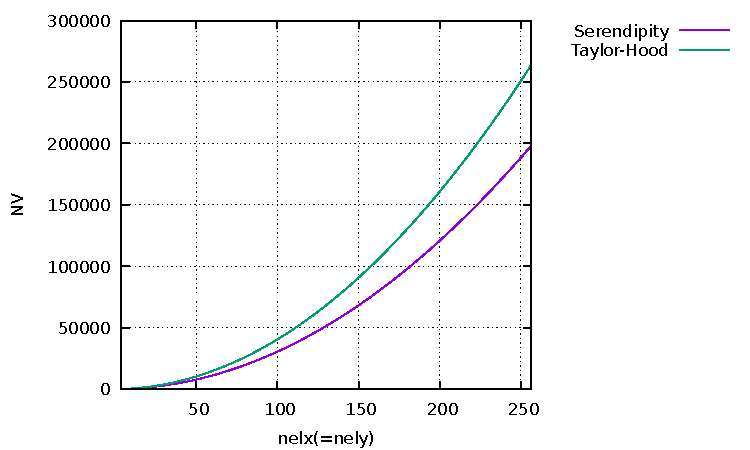
\includegraphics[width=6cm]{python_codes/fieldstone_52/NV.pdf}
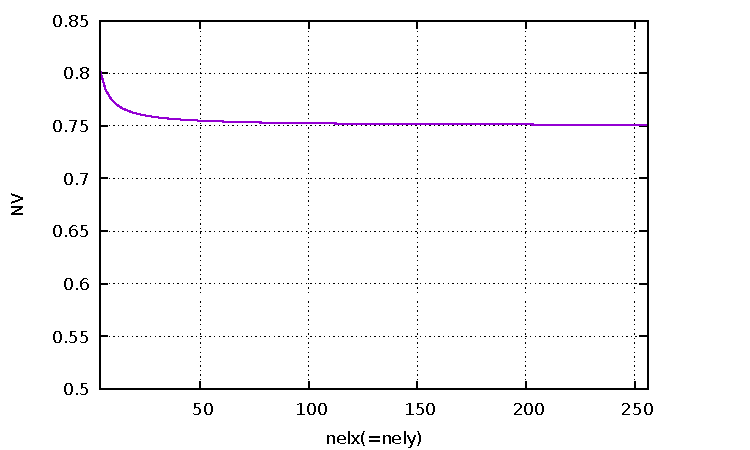
\includegraphics[width=6cm]{python_codes/fieldstone_52/NV_ratio.pdf}
\end{center}
Looking at the ratio between both, we see that ultimately 
at high resolution, a mesh composed of serendipity elements 
will count 25\% less nodes than a mesh with Taylor-Hood elements.
Since there is not free lunch, what is the price paid in terms of accuracy when using 
the cheaper serendipity? 

The shape functions and their derivatives are in Section~\ref{sec:serendipity2D}.

Although the vtk format does not understand the $Q_2$ element in 2D or 3D, it surprisingly does
understand the serendipity element in 2D (type=23) and 3D (type=25).

\begin{center}
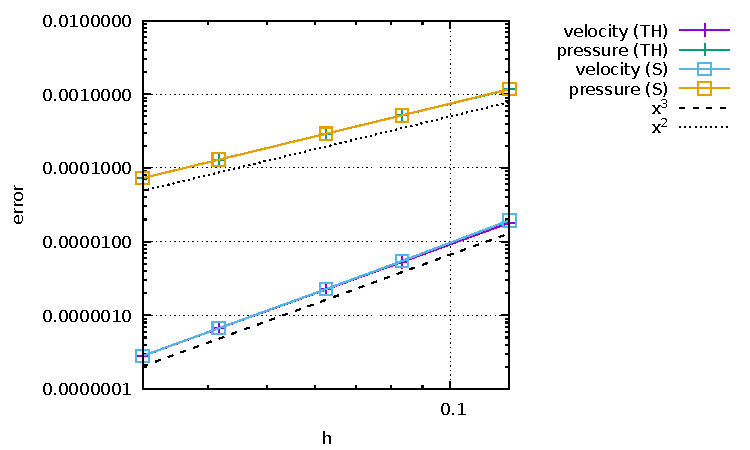
\includegraphics[width=8cm]{python_codes/fieldstone_52/errors.pdf}
\end{center}


